\documentclass[aspectratio=43,unicode,10pt]{beamer}
\usetheme{ttipresentation}

\usepackage{luatexja}
\usepackage{luatexja-fontspec}
\usepackage{graphicx}
\usepackage{multicol}

\setmainjfont{ipagp.otf}
\beamertemplatenavigationsymbolsempty

\newcommand{\itemtitle}[1]{\textbf{#1}\\}
\newcommand{\fire}[1]{\textcolor{red}{\textbf{#1}}}
%\newcommand{\freeze}[1]{\textcolor{blue}{\textbf{#1}}}
\newcommand{\then}{\textcolor{ttiblue}{\textbf{⇒}}\hspace{1ex}}
\newcommand{\good}{\textcolor{orange}{\textbf{◎}}\hspace{1ex}}
\newcommand{\arrow}{\textcolor{ttiblue}{\textbf{→}}\hspace{1ex}}
\newcommand{\mb}[1]{\mathbf{#1}}
\newcommand{\arrowed}[1]{\vec{\mathbf{#1}}}
\newcommand{\term}{終端記号}
\newcommand{\nt}{非終端記号}
\newcommand{\opennt}{openな\nt}
\newcommand{\closednt}{closedな\nt}


\newcommand{\thetitle}{Recurrent Neural Network Grammers}
\title{\thetitle}
\author[Chris Dyer et al.]
       {Chris Dyer, Adhiguna Kuncoro, Miguel Ballesteros, \\ Noah A. Smith}


\newcommand{\bigger}{\Large}

\begin{document}

\begin{frame}
  \titlepage
\end{frame}

\begin{frame}{導入}
  \begin{block}{\thetitle~(RNNGs)}
    \begin{itemize}
      \item 文の確率的生成モデル
        \begin{itemize}
          \item \fire{単語や句の入れ子的・階層的構造を陽に表現}
        \end{itemize}
      \item 問題:構文解析、文生成
      \item 動機:SequentialなRecurrent Neural Networks (RNNs)は \\
            自然言語の潜在的な入れ子構造を考慮できていない
      \item 構成要素
        \begin{itemize}
          \item 構文解析または文生成のアルゴリズム
          \item NNによる生成モデル
        \end{itemize}
    \end{itemize}
  \end{block}
\end{frame}

\begin{frame}{提案手法}
  \begin{block}{RNNGの形式的な定義}
    \begin{gather*}
      RNNG := (N, \Sigma, \Theta) \\
      \begin{cases}
        N: \text{\nt の有限集合} \\
        \Sigma: \text{\term の有限集合} (N \cup \Sigma = \emptyset) \\
        \Theta: \text{NNのパラメータ}
      \end{cases}
    \end{gather*}
  \end{block}
\end{frame}

\begin{frame}{提案手法}
  \begin{block}{構文解析のアルゴリズム}
    \begin{gather*}
      f: X \rightarrow Y \\
      \begin{cases}
        x: \text{\term (単語)の列(入力)} \\
        y: \text{構文木(出力)} \\
        S: \text{スタック} \\
        B: \text{入力バッファ}
      \end{cases}
    \end{gather*}
    \begin{itemize}
      \item スタックの要素:\term、openまたはclosedな\nt
      \item 入力バッファの要素:\term
      \item 初期状態
        \begin{gather*}
          S = \emptyset \\
          B = [T_1, \ldots, T_n] \\
        \end{gather*}
    \end{itemize}
  \end{block}
\end{frame}

\begin{frame}{提案手法}
  \begin{block}{構文解析のアルゴリズム}
    \begin{itemize}
      \item 遷移の制約
        \begin{itemize}
          \item $n$: スタック内の\opennt の数
        \end{itemize}
        \begin{table}
          \begin{tabular}{c | l}
            遷移 & 制約 \\
            \hline
            NT(X)   & $B \neq \emptyset \wedge n < 100$ \\
            \hline
            SHIFT   & $B \neq \emptyset \wedge n \geq 1$ \\
            \hline
            REDUCE  & \parbox{20em}{$
              \text{スタック内の一番上の要素が} \\
              \text{\opennt でない} \\
              \wedge (n \geq 2 (1じゃないの?) \vee B = \emptyset)
            $} \\
          \end{tabular}
        \end{table}
    \end{itemize}
  \end{block}
\end{frame}

\begin{frame}{提案手法}
  \begin{block}{構文解析のアルゴリズム}
    \begin{figure}
      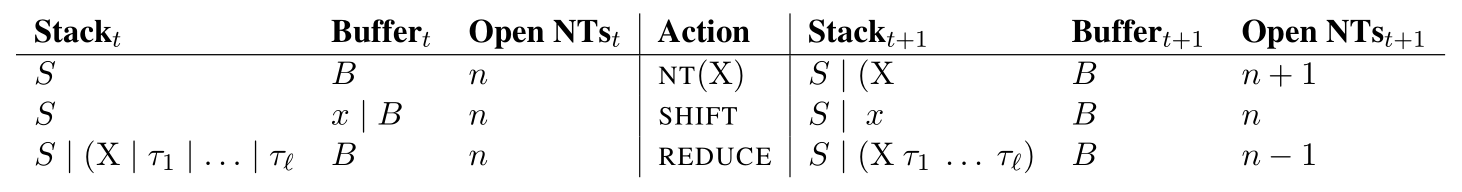
\includegraphics[width=0.9\textwidth]{fig/fig_1.png}
    \end{figure}
    \vspace{-1.5em} % HACK
    \begin{figure}
      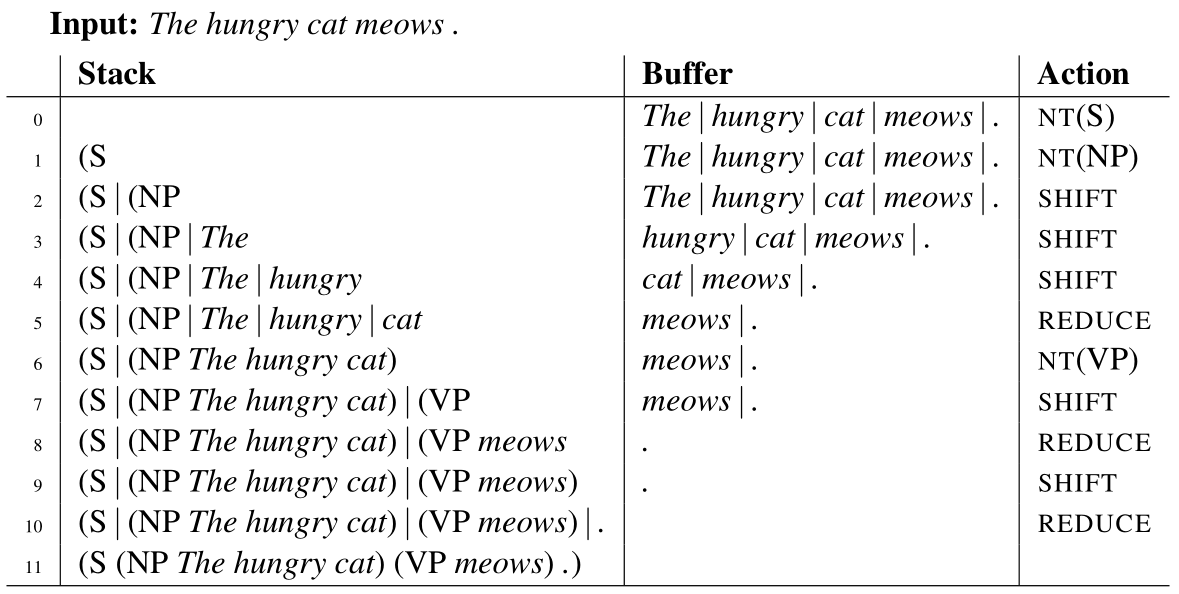
\includegraphics[width=0.9\textwidth]{fig/fig_2.png}
    \end{figure}
  \end{block}
\end{frame}

\begin{frame}{提案手法}
  \begin{block}{文生成のアルゴリズム}
    \begin{gather*}
      f: X \rightarrow Y \\
      \begin{cases}
        x: ? \\
        y: \text{\term (単語)の列(出力)} \\
        S: \text{スタック} \\
        \fire{T: \text{出力バッファ}}
      \end{cases}
    \end{gather*}
    \begin{itemize}
      \item スタックの要素:\term、openまたはclosedな\nt
      \item 出力バッファの要素:\term
      \item 初期状態
        \begin{gather*}
          S = \emptyset \\
          T = \emptyset \\
        \end{gather*}
    \end{itemize}
  \end{block}
\end{frame}

\begin{frame}{提案手法}
  \begin{block}{文生成のアルゴリズム}
    \begin{itemize}
      \item 遷移の制約
        \begin{itemize}
          \item $n$: スタック内の\opennt の数
        \end{itemize}
        \begin{table}
          \begin{tabular}{c | l}
            遷移 & 制約 \\
            \hline
            GEN(X) & $n \geq 1$ \\
            \hline
            REDUCE  & \parbox{20em}{$
              \text{スタック内の一番上の要素が} \\
              \text{\opennt でない} \\
              \wedge n \geq 1
            $} \\
          \end{tabular}
        \end{table}
    \end{itemize}
  \end{block}
\end{frame}

\begin{frame}{提案手法}
  \begin{block}{文生成のアルゴリズム}
    \begin{figure}
        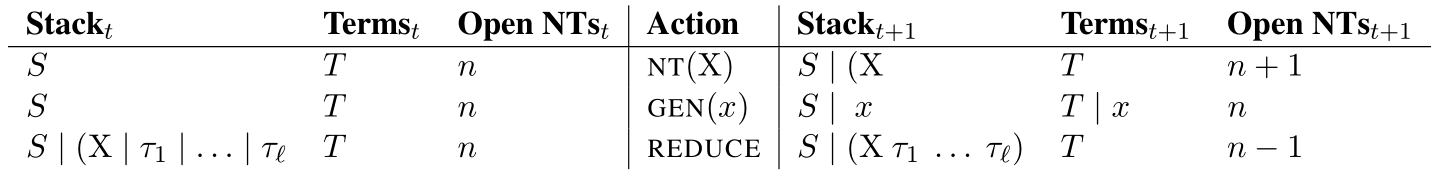
\includegraphics[width=0.9\textwidth]{fig/fig_3.png}
    \end{figure}
    \vspace{-1.5em} % HACK
    \begin{figure}
        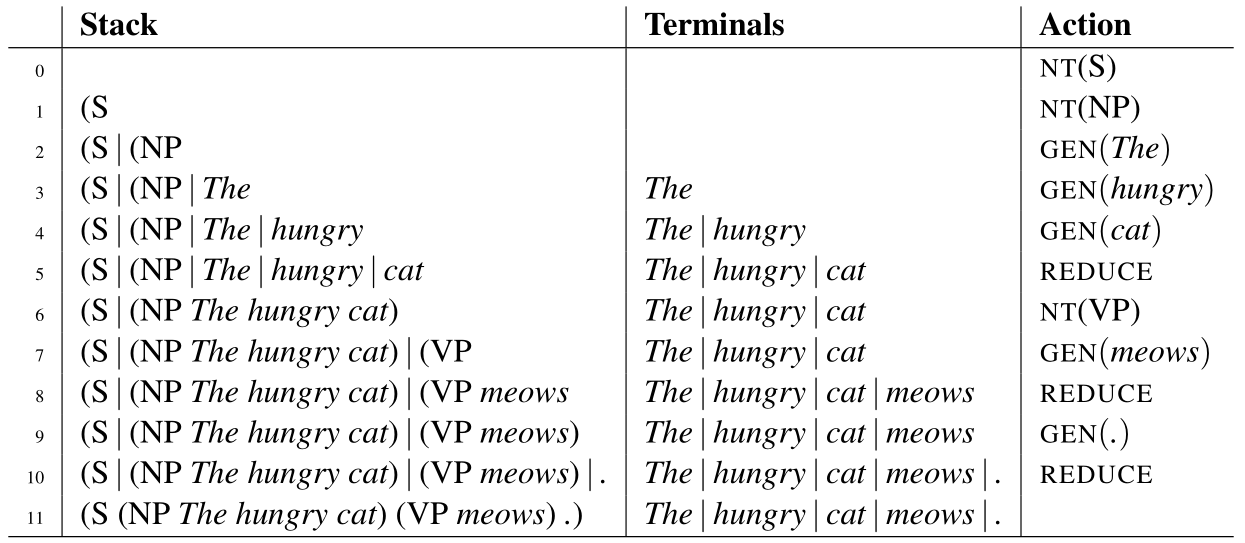
\includegraphics[width=0.9\textwidth]{fig/fig_4.png}
    \end{figure}
  \end{block}
\end{frame}

\begin{frame}{提案手法}
  \begin{block}{生成モデル}
    \begin{itemize}
      \item 単語列($x$)と構文木($y$)の結合確率
    \end{itemize}
    \begin{align*}
      p(x, y) & = \prod_{t=1}^{|a(x, y)|} p(a_t | a_{<t}) \\
              & = \prod_{t=1}^{|a(x, y)|}
                  \frac{\exp r_{a_t}^T u_t + b_{a_t}}
                      {\sum_{a' \in A_G(T_t, S_t, n_t)}
                        \exp r_{a'}^T u_t + b_{a'}} \\
      u_t & = \tanh (W[o_t; s_t; h_t] + c)
    \end{align*}
    \begin{gather*}
      \begin{cases}
        u_t: \text{アルゴリズムの状態を表す埋め込み} \\
        r_a: \text{各遷移の埋め込み(パラメータ)} \\
        b_a: \text{各遷移のバイアス(パラメータ)} \\
      \end{cases}
    \end{gather*}
  \end{block}
\end{frame}

\begin{frame}{提案手法}
  \begin{block}{生成モデル}
    \begin{itemize}
      \item $u_t$: アルゴリズムの状態を表す埋め込み
    \end{itemize}
    \begin{align*}
      u_t & = \tanh (W[o_t; s_t; h_t] + c)
    \end{align*}
    \begin{gather*}
      \begin{cases}
        o_t: \text{出力バッファの状態を表す埋め込み} \\
        s_t: \text{スタックの状態を表す埋め込み} \\
        h_t: \text{遷移歴を表す埋め込み} \\
        W, c: \text{パラメータ}
      \end{cases}
    \end{gather*}
  \end{block}
\end{frame}

% \begin{frame}{\thetitle}
%   \only<1>{
%     \begin{itemize}
%       \bigger
%       \item タスク:商品レビューの\fire{レーティング予測}
%       \item \fire{レビュー解析}:レビューのどの部分が重要か
%     \end{itemize}

%     \begin{figure}
%       \includegraphics[width=0.8\linewidth]{fig/review.pdf}
%     \end{figure}
%   }

%   \only<2>{
%     \begin{itemize}
%       \bigger
%       \item 対象言語:以下の種類の文字を含む言語
%     \end{itemize}
%     \begin{figure}
%       \includegraphics[width=0.75\linewidth]{fig/logogram_and_ideogram.pdf}
%     \end{figure}
%     \begin{itemize}
%       \bigger
%       \item モデル: \fire{フォント画像} \arrow 文字埋め込み \\
%                     \arrow 単語、文、文書埋め込み \arrow レーティング
%     \end{itemize}
%   }

%   \only<3>{
%     \begin{itemize}
%       \bigger
%       \item 解析結果
%     \end{itemize}
%     \begin{figure}
%       \includegraphics[width=0.8\linewidth]{fig/review_1.png}
%     \end{figure}\vspace{-2ex} % HACK
%     \begin{figure}
%       \includegraphics[width=0.7\linewidth]{fig/review_2.png}
%     \end{figure}
%   }
% \end{frame}

\end{document}
